\documentclass[runningheads,a4paper]{llncs}

\usepackage{amssymb}
\setcounter{tocdepth}{3}
\usepackage{graphicx}

\usepackage{url}
\newcommand{\keywords}[1]{\par\addvspace\baselineskip
\noindent\keywordname\enspace\ignorespaces#1}

% Additional packages
\usepackage[utf8]{inputenc}
\usepackage{subfig}
\usepackage[pdftex,pdfpagelabels,bookmarks,hyperindex,hyperfigures]{hyperref}
\hypersetup{%
   plainpages=false, 
   pdfpagelayout=SinglePage,
   bookmarksopen=false,
   bookmarksnumbered=true,
   breaklinks=true,
   linktocpage,
   colorlinks=true,
   linkcolor=blue,
   urlcolor=blue,
   citecolor=blue,
   anchorcolor=green
}      

\begin{document}

\mainmatter  % start of an individual contribution

% first the title is needed
\title{Novelty Detection Using Graphical Models for Semantic Room Classification}

% a short form should be given in case it is too long for the running head
% \titlerunning{Lecture Notes in Computer Science: Authors' Instructions}

% the name(s) of the author(s) follow(s) next
%
% NB: Chinese authors should write their first names(s) in front of
% their surnames. This ensures that the names appear correctly in
% the running heads and the author index.
%
\author{André Susano Pinto}
%
%\authorrunning{Lecture Notes in Computer Science: Authors' Instructions}
% (feature abused for this document to repeat the title also on left hand pages)

% the affiliations are given next; don't give your e-mail address
% unless you accept that it will be published
\institute{Faculdade de Engenharia da Universidade do Porto, Portugal\\
\url{andresusanopinto@gmail.com}\\
\url{http://url}}

\toctitle{Lecture Notes in Computer Science}
\tocauthor{Authors' Instructions}
\maketitle


\begin{abstract}
This paper presents an approach to the problem of novelty
detection in the context of semantic room categorization.
The ability to assign semantic labels to areas in the environment is crucial for
autonomous agents aiming to perform complex human-like tasks and human
interaction.
However, in order to be robust and naturally learn the semantics from
the human user, the agent must be able to identify gaps in its own knowledge.
To this end, we propose a method based on graphical models to identify novel
input which does not match any of the previously learnt semantic descriptions.
The method employs a novelty threshold defined in terms of conditional
and unconditional probabilities. The novelty threshold is then optimized using
an unconditional probability density model trained from unlabelled data.


\keywords{novelty detection, semantic data, probabilistic graphical models,
room classification, indoor environments, robotics, multi-modal classification.}
\end{abstract}


%%%%%%%%%%%%%%%%%%%%%%%%%%%%%%%%%%%%%%%%%%%%%%%%%%%%%%%%%%%%%%%%%%%%%%
\section{Introduction}
There has been several efforts in the area of Artificial Intelligence and Robotics
in creating robots that are able to interact with humans and their environments.
One of the existing problems is a reliable high-level localization method that can
be deployed into new and unknown environments or where its impossible to access a
previously labelled map of the area. Nonetheless the need of reliability and ability
to deal with new cases also arises due to dynamic changes on the environment through
time and with human action.
This article focus on the mapping, using \emph{semantic data}, of indoor
environments such as houses and offices to room categories such as kitchen,
corridor, office.

Due to the unknown and dynamic nature of the operating environment the
mapping methods should be resilient to new room categories the agent has never seen
before. This is: perform novelty detection on the concepts the agent is aware of.

Dora\cite{dora} (CogX: Dora) was used as a base system where to implement the
presented novelty detection system as it already possesses a developed architecture
oriented on dealing with probabilistic and semantic information and performing
reasoning over it.
Implementing novelty detection capabilities on an agent such as Dora, would allow to
to increase reliability and allow the creation of self-extending behaviours.

Its with a final interest on integrating the developed methods on Dora that this
initial work focus on the novelty detection using probabilistic graphical models
that model the conceptual knowledge and information handled by Dora.


%%%%%%%%%%%%%%%%%%%%%%%%%%%%%%%%%%%%%%%%%%%%%%%%%%%%%%%%%%%%%%%%%%%%%%
\section{Related Work}
% TODO(pronobis): general comment about many .... approches to place categorization.
The problem of room categorization based on visual information was first addressed
in the computer vision community. In this case, the research focused mainly on the
problem of classifying single images captured in indoor or outdoor environments
(scene classification). At the same time, robotics researchers initially employed
the 2D laser range sensor being much more robust to variations occurring in the
environment and much easier to handle computationally in real time.

Multi-modal approaches, such as combining semantic data extracted from
several sources or classifiers are expected to have better performance on scene
recognition than single-cue approaches. Quattoni and Torralba\cite{quattoni2009recognizing}
showed that most scene recognition models work poorly in indoor scenes when
compared to outdoor scenes since the properties that
characterize rooms changes depending on the category. For instance corridors are well
described by global properties and bookstores are well described by the presence of
specific objects (books).
Galindo et al.\cite{galindo2005multi} also exploits this by defining a bidirectional relation
between object and room category, where object defines a room category and a room
category provides information on where objects may be found.

Probabilistic representations have been frequently used for spatial modelling
in robots operating in the real-world\cite{gross2009toomas,maierprobabilistic}.
Boutell et al.\cite{boutell2006factor} have studied outdoor scene classification using
\emph{factor graphs} and modelling spatial relations between objects in the scene
to extract better knowledge from semantic (high-level) features.

Although our approach is presented in the context of mobile robotics it relies on
standard concepts and techniques such as semantic data and graphical models.
Those are often used in the area of information retrieval.
An interesting example is the usage of an hidden concept layer between visual features
and text information to provide automatic image annotation\cite{zhang2005probabilistic}.

Novelty detection has been studied for many years and there are several approaches
based on statistical analysis\cite{markou2003novelty}.
Graphical models have been used to learn distributions of variables, both in
supervised and unsupervised ways and by using thresholds on those distributions
based solely on the conditional probability as seen on Bishop\cite{bishop1994novelty}
a novelty system can be trivially implemented.

However to the knowledge of the authors there is no reference on how to perform
novelty detection using graphs that are dynamically generated.
% TODO(andresp): anything more that can be said on why this paper is useful?

%%%%%%%%%%%%%%%%%%%%%%%%%%%%%%%%%%%%%%%%%%%%%%%%%%%%%%%%%%%%%%%%%%%%%%
\section{Dora Architecture Overview}
Short paragraph describing dora. Short paragraph describing dora. Short paragraph describing dora. Short paragraph describing dora. Short paragraph describing dora.

As Dora moves through the environment its \emph{conceptual layer} builds a structural and
probabilistic representation of the space instantiated as a \emph{graphical model}.
That model connects the sensed properties together with the variables used to model the world.
And allows to perform queries on the probabilities of aspects of the environment.
For example: where is most likely to find a cereal box\cite{exploiting}.

From its architecture only the \emph{conceptual layer} is of interest to this article.
Its role is to aggregate the following semantic information coming from other layers:

\begin{description}
 \item[Doorway detection] is used to segment the low-level space into rooms and map connectivity between them.
 \item[Room size and shape] are classified by using 2D laser scans data and are associated as properties of a given room. The system utilizes pre-trained set of classifiers to label size as (large, medium, small) and shape as (rectangular or elongated).
 \item[Object detection] is performed using the visual input in order to detect . The system keeps track of the number of object and types seen per each room. Objects are once again detected by running a pre-trained set of detectors for: book, cereal box, computer, robot, stapler, toilet paper.
 \item[Room appearance] is categorized from the visual input by using CRFH and a pre-trained set of 7 different models.
\end{description}

With the extracted information and conceptual knowledge the conceptual layer creates a structured probabilistic representation
in order to model all known variables and their relations.
As so, in order to represent the knowledge the layer builds a \emph{chain graph}:
a probabilistic graphical model that merges both Bayesian Networks and Random Markov Fields.

The use of graphical models to describe distributions of variables has useful properties.
The edges between the variables can be seen as a kind of filter to the properties of the system.
Properties those that are expected to be captured by the conceptual knowledge.
At the same time they are a generative models and therefore allow to calculate the probability
on any given subset of variables on the graph allowing the system to work even when some
information is missing.

\begin{figure}[h]
\centering
\subfloat[Conceptual layer]{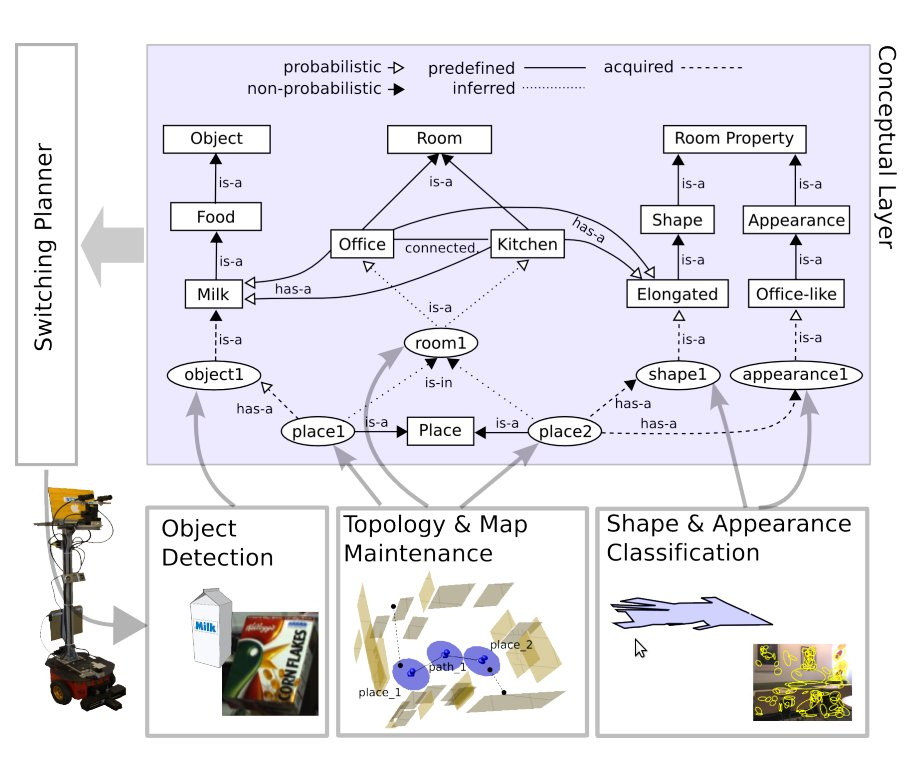
\includegraphics[width=0.50\textwidth]{figures/conceptual-layer.jpg}}
\subfloat[Chain graph]{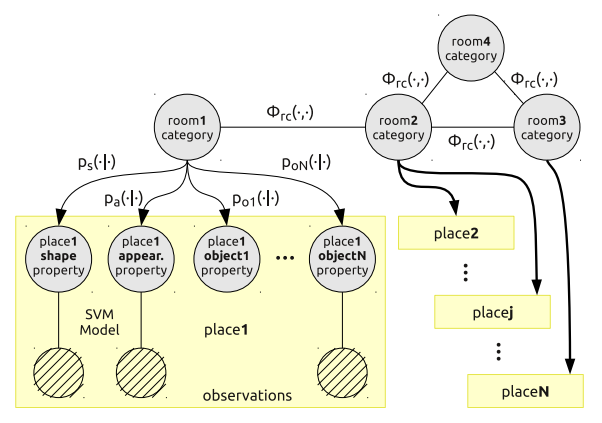
\includegraphics[width=0.49\textwidth]{figures/chain-graph.png}}

\caption{The conceptual layer structures the sensed environment together with the conceptual knowledge
         in order to create a structured probabilistic representation of the world.}
\end{figure}

\subsection{Factor Graphs}
Although the conceptual layer works with \emph{chain graphs}, those can be converted
into \emph{factor graphs}\cite{kschischang2001factor}. Factor graphs are used throughout this paper as they provide an
easier manipulation due to factorization.
Moreover, there exists efficient implementation of inference engines operating on factor graph
representations\cite{Mooij_libDAI_10}.
Describing the distribution function in terms of graphs allows to use those engines to
efficently calculate marginals on any given subset of variables by exploiting conditional
independence between variables.

A \emph{factor graph} is a bipartite graph connecting two sets of nodes $X_G$ and $F_G$
representing random variables and factors.
Each factor is described by function $\phi$ dependent only on the variables $x_\phi$
to which the factor is connected.
Thus, a factor graph can be seen as a description of probability density function obtained
by a product of all the factors. In order to represent the probability,
a normalization factor needs to be introduced, resulting in the following equation:

\begin{equation}
P_G(x) = \frac{1}{Z}\prod_{\phi \in F_G}{\phi(x_{\phi})},\qquad
Z = \sum_{X_G}\prod_{\phi \in F_G}{\phi(x_{\phi})}
\end{equation}


%%%%%%%%%%%%%%%%%%%%%%%%%%%%%%%%%%%%%%%%%%%%%%%%%%%%%%%%%%%%%%%%%%%%%%
\section{Novelty Detection}
% Introduce novelty detection
Novelty detection deals with detecting that a new input was generated by a class
other than the ones the system knows about\cite{markou2003novelty}.
It is harder than classification as only positive samples of a class are available
rendering normal classification methods invalid.

% Explain threshold approach to novelty detection
Due to the desire of robustness, a novelty detection system would
always possess some threshold that describes on how strict the system should be to
new samples. This threshold describes a trade between error and rejection: as the
more the system tries to reduce rejection the more prone to produce
errors it becomes.
This threshold if often seen as a max allowed distance between a sample and the known
class.

When dealing with a statistic point of view, noisy data or unstable features, a decision to
classify a sample as novel as an associated error probability of $P(\overline{novel}|x)$.
And the error rate of a system that classifies the set of inputs $N$ as novel is given by
the equation:

\begin{equation}
P(e) = \frac{\sum_{n \in N}{P(\overline{novel}|n)P(n)}}{\sum_{n \in N}{P(n)}}
\end{equation}

Therefore any novelty system that decides to acknowledge a sample
$a$ as novel should also detect novelty on any sample $b$ satisfying
$P(\overline{novel}|b) < P(\overline{novel}|a)$.
As that would always reduce the error probability.
This way a novelty detection system is interested in defining an
order on all the possible inputs equivalent to the order defined by
the error rate: $P(\overline{novel}|x)$.

Using Bayes rule and assuming a constant $P(\overline{novel})$
a ratio between a conditional and unconditional probabilities of the input $x$ is obtained.
Such a ratio is a suitable function for implementing a novelty detector system with optimal
thresholding.

\begin{equation}
\label{eq:novelty-threshold}
          P(\overline{novel}|x)
  =       \frac{P(x|\overline{novel}) P(\overline{novel})}{P(x)}
  \propto \frac{P(x|\overline{novel})}{P(x)}
\end{equation}

% Explain approach of using conditional probability
\subsection{Conditional Probability}
\label{sec:conditional-prob}


In the presented case the conditional probability is approximated by the graphical model $G$
produced by the conceptual layer.
\autoref{fig:conditional-prob-graph} represents a possible graph $G$ built from the conceptual
layer to represent the conditional probability on the sensed variables $x$.
$P_G(x)$ is used as an approximation for $P(x|\overline{novel})$.

\begin{figure}[h]
\centering
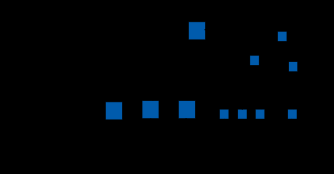
\includegraphics[width=0.70\textwidth]{figures/conditional-prob-graph.pdf}
\caption{\label{fig:conditional-prob-graph}The conceptual layer models the conditional
         probability distribution of the sensed variables by using hidden variables.
         Those are created from the conceptual knowledge and represent the structural
         and connectivity information the system is aware of.
         In this case only hidden variables $R_i$ were used to model the room categories
         where each property was sensed.}
\end{figure}

\subsection{Unconditional Probability}
\label{sec:unconditional-prob}
One of the hardest problems is that on most cases a novelty detection system only
has access to the known data.
Under that the best approach is to define a threshold assuming that $P(x)$ is
constant through all the input space.

Its important to notice that in several cases assuming it to be constant leads to
discarding the factor.
Nonetheless, here the distributions are dynamically changing as the system learns
more on the environment.
So the normalizing argument $P(x)$ has to be evaluated for each new subset of $x$.

Assuming that the unconditional distributions generates all possible outcome with
the same probability we can model it with $\prod{1/\# x_i}$,
where $\# x_i$ denotes the cardinality of the state space of variable $x_i$.
In graphical model terms this is represented to a factor graph $U$ with the
variables but without any factors as illustrated on \autoref{fig:uniform-prob-graph}.

\begin{figure}
\centering
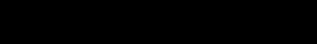
\includegraphics[width=0.70\textwidth]{figures/uniform-prob-graph.pdf}
\caption{\label{fig:uniform-prob-graph}Without any existing factors, this graph $U$ represents a
         uniform distribution over any set of its variables.}
\end{figure}

Having a graphical model $G$ built to model the known data distribution and a model
$U$ for the unconditional probability a novelty threshold would be given by:
$P_G(x)/P_U(x)$.
Here $P_{U}(x)$ can be seen as a normalizing factor to lever all the $P_G(x)$ on any set of
variables $x$ into the same measure units (error rate), such that a static threshold can be implemented.
For example the conditional probability would yield very small values on large sets of variables
$x$ than in small sets due to the spreading over the dimensions of the input space.
As so a novelty measure is seen as a ratio on how much introducing the known concepts helps to
understand the observed result.


\subsection{Semi Supervised: Using Unlabelled Data}
Nonetheless its often the case that there is access to large amounts of unlabelled data.
Under that it becomes possible to obtain a better approach to the unconditional probability
distribution than the uniform one.

For interesting and practical reasons it was assumed that the unconditional distribution
could be modelled with all the variables independent from each other.
Which translates as $P(x)=\prod{P_{x_i}(x_i)}$.
From the unlabelled data only the probability of each feature $x_i$ needs to be estimated.
\autoref{fig:semisupervised-threshold} illustrates a graph $I$ to model independent variables.

\begin{figure}[h]
\centering

\includegraphics[width=0.70\textwidth]{figures/independent-prob-graph.pdf}
\caption{\label{fig:semisupervised-threshold}Using unlabelled data, its possible to estimate
         the unconditional probability for each variable and this way try to compensate
         for a possible existent bias on some of the variables.}
\end{figure}

Once again the novelty threshold would be given by $P_G(x)/P_I(x)$.
This time the addition of the variables unconditional factors can be understood as an
attempt to compensate for an existing bias on the unconditional distribution.
Which is an important step to achieve a correct ordering of the input space for novelty
thresholding.


%%%%%%%%%%%%%%%%%%%%%%%%%%%%%%%%%%%%%%%%%%%%%%%%%%%%%%%%%%%%%%%%%%%%%%
\section{Results}
In order to verify the performance of the proposed thresholds a synthetic dataset
was generated. To keep it simple only information regarding direct properties of
a room were modelled and no structured knowledge such as room connectivity was taken
in account.
The synthetic distribution assumes that an independent and variable size set of features
$x$ is generated by a given room category.
In whole there was 11 different room categories and 7 different measured feature
types. Each feature type can be present more than once in (Eg.: room shape is
extracted from 2D laser scans in more than one position in the room).

The room categories were chosen to mimic as close as possible real features and
categories existent on reality. And they model different room categories with
different levels of detail. For example: 1 person office, 2 person office, hallway,
robot lab.

From the distribution, 100 labelled samples for 5 of the 11 room categories were
drawn to represent the known concepts and 1000 unlabelled samples were drawn from
all the room categories for learning the unconditional probability distribution.
Using those samples, factors were learnt for the graphs used to model the
conditional distribution and the independent unconditional distribution.
\autoref{fig:simple-experiment} shows the graph structure used for approximate the
trained conditional and unconditional distributions.
Its important to notice that graph $G$ used to model the known classes perfectly
mimics the real distribution, with the exception that the system is not aware of
all the room categories.

\begin{figure}[h]
\centering

\subfloat[Graph structure $G$.]{
         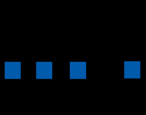
\includegraphics[width=0.27\textwidth]{figures/simple-cond-graph.pdf}}
\qquad
\subfloat[Graph structure $U$.]{
         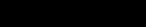
\includegraphics[width=0.27\textwidth]{figures/simple-uniform-graph.pdf}}
\qquad
\subfloat[Graph structure $I$.]{
         
\includegraphics[width=0.27\textwidth]{figures/simple-independent-graph.pdf}}

\caption{\label{fig:simple-experiment}The graph structures used to model the
         conditional and unconditional probability for implementing the novelty
         thresholds $P_G(x)/P_U(x)$ and $P_G(x)/P_I(x)$.}
\end{figure}

% Describe how to obtain the 3 thresholds functions seen on the graphs.
Using the learned models $G$, $U$ and $I$ two thresholds were trained:
$P_G(x)/P_U(x)$ assuming a uniform unconditional distribution
and $P_G(x)/P_I(x)$ assuming an independent unconditional distribution.
Since the distribution is synthetic there is access to $P(x)$ and $P(x|concept)$
and so a perfect threshold function could also be created to test how far the
presented thresholds are from optimal.

\subsection{Probability ratio comparison}
%%% Results 1
% Show the threshold ratio is an optimal detector (if perfect information was available)
% Show that the thresholds are suitable functions for implementing a static threshold.
As first tryout, the performance of the novelty thresholds was plotted for a set
of 1000 samples taken out from the whole distribution (\autoref{fig:synthetic-roc}).
Those samples contain different number of sensed properties for each room, miming
the dynamic properties expected to see when implemented on a robot.

\begin{figure}[h]
\centering
\includegraphics[width=0.60\textwidth]{results/synthetic-all.pdf}

\caption{\label{fig:synthetic-roc}ROC curve comparing novelty detection performance
         under samples with variable size of sensed properties.}
\end{figure}

The convex shape of the optimal threshold shows that the ratio between conditional
and unconditional probability is indeed an optimal detector and is suitable for
implementing a static threshold when the samples are taken from dynamic
distributions (eg.: some samples where there is only access to room size versus
samples where there is a lot of information on the room properties).

% Discuss importance on approximating unconditional probability.
Its also possible to see how important it is to estimating a correct unconditional
probability in order to obtain a correct novelty ordering on the inputs.
The assumption of an uniform unconditional probability has led to very poor results.
That is probably explained by semantic properties as the ones modelled to be highly
biased towards some values and understanding that bias plays an important step
to detect whether a given sensed value is a valuable clue on the room category
or not.



%%% Results 2
% Measure performance of the thresholds as more information becomes available.
\subsection{Performance changes with amount of available information}
In order to measure the performance impact as more semantic information becomes
available ROC curves were plotted for samples grouped by the number of sensed
semantic features.

\begin{figure}[h]
\centering

\subfloat[3 sensed features]{\includegraphics[width=0.40\textwidth]{results/synthetic-3features.pdf}}
\qquad
\subfloat[5 sensed features]{\includegraphics[width=0.40\textwidth]{results/synthetic-5features.pdf}}

\subfloat[10 sensed features]{\includegraphics[width=0.40\textwidth]{results/synthetic-10features.pdf}}
\qquad
\subfloat[50 sensed features]{\includegraphics[width=0.40\textwidth]{results/synthetic-50features.pdf}}

\caption{\label{fig:synthetic-roc-breakdown}ROC curves plotted showing performance of the
         presented novelty detection method on graphs generated for different amount of
         sensed features.}
\end{figure}

As possible to see as the system gains more semantic information it becomes easier
to detect novelty as the input space size increases and allows the several existing
classes to become more easily distinguished.

The performance of the independent threshold decreases as the number of sensed
features increases. This is easily explained by the fact that the graph $I$ is not
able to model the existent dependence between the features and that becomes obvious
as the number of features increases (Eg.: graph $I$ perfectly models $P(x)$ in the
case where only 1 feature is sensed).

The uniform threshold shows a very poor performance specially on small size samples
where its performs almost no better than random.
It performance increases as the size of sensed features increases but nonetheless
its always very small when compared to how optimal a threshold could be.
This shows that at least under semantic distributions as the one modelled with the
synthetic data assuming an uniform unconditional distribution leads to poor results.


%%%%%%%%%%%%%%%%%%%%%%%%%%%%%%%%%%%%%%%%%%%%%%%%%%%%%%%%%%%%%%%%%%%%%%
\section{Conclusions and Future Work}
In this paper we presented how to define a stable novelty threshold function on
top of \emph{probabilistic graphical models} instantiated dynamically from sensed
semantic data.
The presented technique is based on the ratio between a conditional and
unconditional probability and when perfect information exists it performs an optimal
novelty detection threshold.

It was also shown that a correct estimation of unconditional probability plays an
important role specially on small input spaces. Moreover, semi-supervised techniques
implemented with the access to unlabelled data can be used to significantly improve
novelty detection performance.

Given the synthetic distribution, an assumption on an uniform
distribution has led to very poor results. The same behaviour is expected to
in real world distributions based on semantic data. For that reason,
and due to easy access to unlabelled data, special attention will be given to using
semi-supervised techniques for novelty detection.

After this initial study on how to detect new semantic classes based on
graphical models, future work will focus on how to use the structured
information available from the conceptual layer to be able to detect which variable
of the graph is novel and what makes it different from other previously learned
classes. That will lead to generation of useful information that can be used for
communication with the user and performing active learning of new room categories.


%%%%%%%%%%%%%%%%%%%%%%%%%%%%%%%%%%%%%%%%%%%%%%%%%%%%%%%%%%%%%%%%%%%%%%
\bibliographystyle{unsrt}
\bibliography{refs}

\end{document}
